\documentclass[a4paper]{jarticle}

\usepackage[top=2cm,bottom=2cm,left=2cm,right=2cm]{geometry}

 \usepackage{url}
 \usepackage[dvipdfmx]{graphicx}

\renewcommand\thefootnote{*\arabic{footnote}}

\newcommand{\resp}[1]{\begin{flushright}文責: #1\end{flushright}~\\ }

\title{Unity班 活動報告書}
\author{立命館コンピュータクラブ\\2021年度プロジェクト活動}
\date{2021年2月8日}

\begin{document}

  \maketitle
  \begin{center}
    % 名前 \footnote{所属学部 所属学科 (あれば所属コース) 回生}というように記述
    堀越 俊行\footnote{情報理工学部 情報理工学科 システムアーキテクトコース 三回生}
        新藤 尚輝\footnote{情報理工学部 情報理工学科 実世界情報コース 二回生}
        宇佐 基史\footnote{理工学部 ロボティクス科 二回生}

    原 佑馬\footnote{情報理工学部 情報理工学科 システムアーキテクトコース 三回生}
      北村 優奈\footnote{情報理工学部 情報理工学科 システムアーキテクトコース 三回生}
        中山 凌一\footnote{情報理工学部 情報理工学科 システムアーキテクトコース 三回生}

    服部 瑠斗\footnote{情報理工学部 情報理工学科 知能情報コース 三回生}
      岡本 陽太\footnote{情報理工学部 情報理工学科 実世界情報コース 三回生}
        桐井 優実\footnote{情報理工学部 情報理工学科 システムアーキテクトコース 二回生}

    中川 拓海\footnote{情報理工学部 情報理工学科 セキュリティ・ネットワークコース 三回生}
        伊藤 佑\footnote{}
        山本 京介\footnote{情報理工学部 情報理工学科 システムアーキテクトコース 一回生}

  \end{center}

  \newpage

  \tableofcontents

  \newpage

  \section{Unity班について}
    \resp{宇佐 基史}
    
  \section{活動について}
    \resp{北村 優奈,原 佑馬}

 \subsection{個人の作成物紹介}
   ここでは,個人の作成物の紹介を行います.

   \subsubsection{3Dアクションゲーム}
        \resp{新藤 尚輝}
        私は,基本的な機能を備えている3DCGを用いたアクションゲームを作成した.\\
        このゲームは,主に以下のオブジェクトから作成されている.
        \begin{quote}
          \begin{itemize}
            \item DreamForestTree(地形)
            \item unitychan(プレイヤー)
            \item ZombiCartoon(敵キャラクター)
          \end{itemize}
        \end{quote}
        上記の三つは共にunityの「Asset Store」からお借りしたものである.また,このゲームには一部効果音・BGMが入っている.それらについて,以下に箇条書きにする.BGMは「魔王魂」,SEは「無料効果音で遊ぼう!効果音検索」からお借りした.\\
        \begin{quote}
          \begin{itemize}
            \item ファンタジー15(BGM)
            \item ファンタジー13(BGM)
            \item short\_punch1(SE)
            \item kick1(SE)
          \end{itemize}
        \end{quote}
        
        このゲームは,以下のボタンを用いて操作する.\\
        \begin{quote}
          \begin{itemize}
            \item ジャンプ(〇ボタン)
            \item 画面遷移(Optionsボタン)
            \item 攻撃(R1ボタン)
            \item スライディング(×ボタン)
            \item ロックオン(R3押し込み)
            \item カメラ操作(Rスティック)
            \item 移動(Lスティック)
          \end{itemize}
        \end{quote}
        
        図1は,タイトル画面である.この画面で,Optionsボタンを押すと,ゲームが開始する.\\
        \begin{figure}[h]
          \centering
          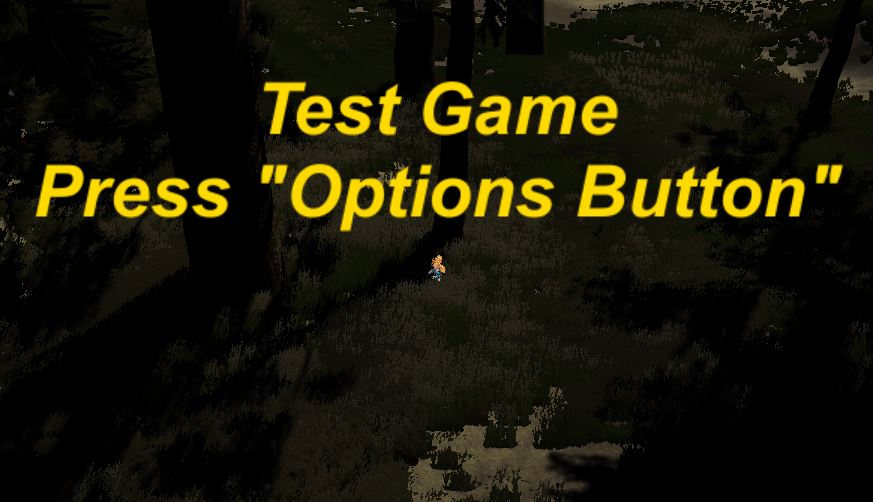
\includegraphics[keepaspectratio, scale=0.5]
               {images/Shindo/start.JPG}
          \caption{タイトル画面}
         \end{figure}
         
         このゲームは敵キャラクターを10体倒すとゲームクリアとなる.図2の画像が,クリア画面である.\\
		\begin{figure}[h]
          \centering
          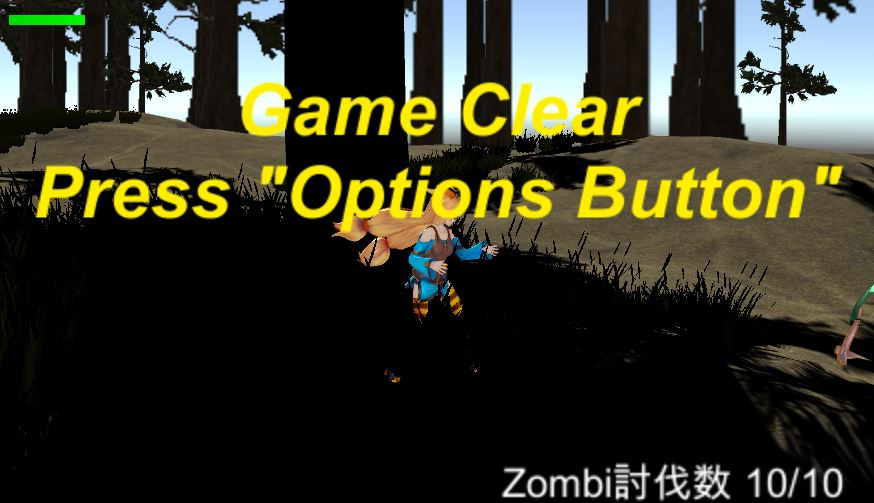
\includegraphics[keepaspectratio, scale=0.5]
               {images/Shindo/clear.JPG}
          \caption{クリア画面}
         \end{figure}
        
         また,操作キャラクターのHPが0になると,ゲームオーバーとなる.図3の画像が,ゲームオーバーの画面である.
         この状態でPS4のoptionsボタン押すと、図1のタイトル画面に戻る.\\
        \begin{figure}[h]
          \centering
          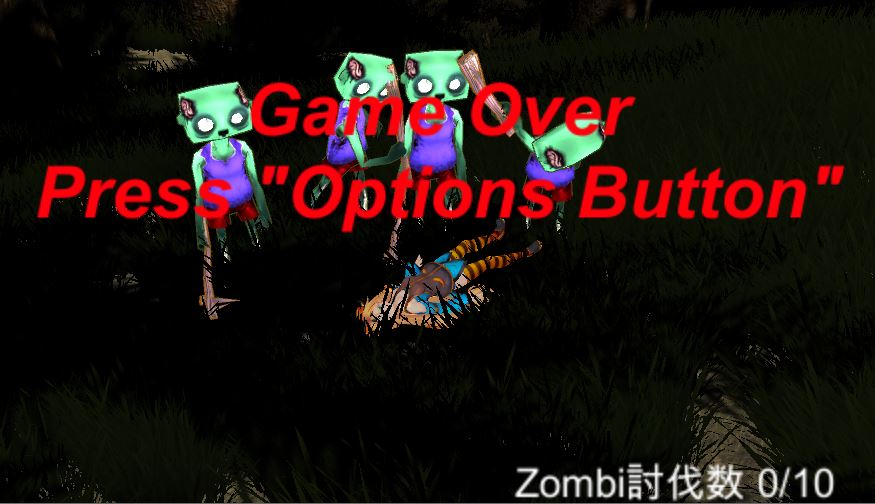
\includegraphics[keepaspectratio, scale=0.5]
               {images/Shindo/gameover.JPG}
          \caption{ゲームオーバー画面}
         \end{figure}
         以上のような流れで,このゲームが進行する.
        
        

 \subsection{年間の活動の上での問題点}
      \resp{山本 京介}
     
    \subsection{年間の活動で得られた知見}
      \resp{桐井 優実}

    \subsection{班総括}
      \resp{新藤 尚輝}
  
\end{document}